% Define block styles
\tikzstyle{block} = [thick, rectangle, draw, text width=3em, text centered, rounded corners, minimum height=3em, fill=black!30]
\tikzstyle{line} = [draw, -latex]
\tikzstyle{dot} = [circle, draw, inner sep=1pt, fill=black]
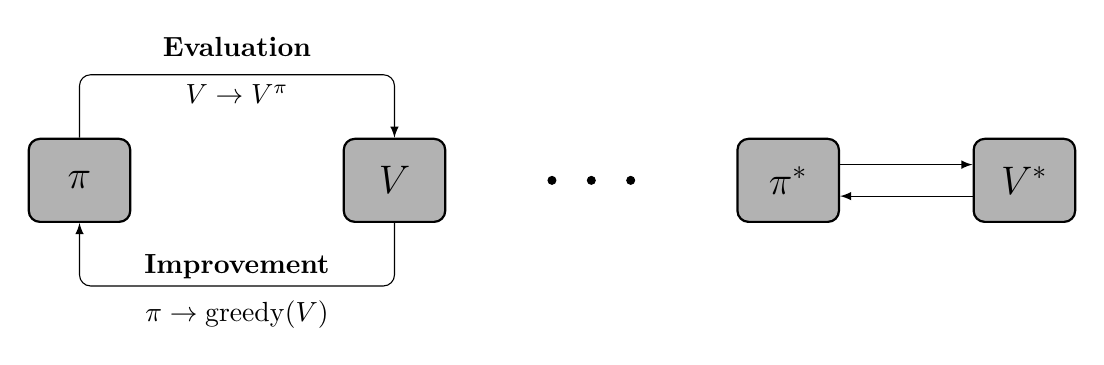
\begin{tikzpicture}[rounded corners]

	% Place nodes
	\node at(-2,0) [block](pie){\Large $\pi$};
	\node at(2,0) [block](vee){\Large $V$};
	\node at(7,0) [block](pie0){\Large $\pi^*$};
	\node at(10,0) [block](vee0){\Large $V^*$};
	
	\path[line] (pie.north) |- ([yshift=0.8cm]vee.north) -- (vee.north);
	\path[line] (vee.south) |- ([yshift=-0.8cm]pie.south) -- (pie.south);
	\path[line] ([yshift=0.2cm]pie0.east) -- ([yshift=0.2cm]vee0.west);
	\path[line] ([yshift=-0.2cm]vee0.west) -- ([yshift=-0.2cm]pie0.east);
	
	\node at (4,0)[dot]{}; \node at (4.5,0)[dot]{}; \node at (5,0)[dot]{};
	
	\node at (0,1.7){\textbf{Evaluation}};
	\node at (0,1.1){$V \rightarrow V^\pi$};
	\node at (0,-1.1){\textbf{Improvement}};
	\node at (0,-1.7){$\pi\rightarrow\mathrm{greedy}(V)$};

\end{tikzpicture}
